
\documentclass[a4paper]{article}
\usepackage[utf8]{inputenc}
\usepackage{graphicx} % Required for inserting images
\usepackage[italian]{babel}
\usepackage{textcomp, gensymb}
\usepackage{array}
\usepackage{amsmath}
\usepackage{hyperref}
\usepackage{siunitx}
\usepackage{caption}
\usepackage{systeme}
\usepackage{wrapfig}
\usepackage[margin=3.25cm]{geometry}
\usepackage{placeins}
\usepackage{float}

\makeindex
\setlength{\parindent}{0pt}

\title{Misura del Modulo di Coulomb usando un Cavo di Acciaio}
\author{Francesco Giuliano Rossi}
\date{Maggio 2025}

\begin{document}
\maketitle
\tableofcontents

\begin{abstract}
In questa esperienza si vuole misurare il modulo di Coulomb per un filo di acciaio. Usando un apparato chiamato il pendolo torcente, possiamo misurare tutto ciò che serve per calcolare il modulo di Coulomb. Questa esperienza è stata fatta nello stesso giorno di quella della misura del Modulo di Young. 
\end{abstract}

\section{Introduzione Teorica}
\subsection{Introduzione Generale}
Ogni materiale, se sottoposti a sollecitazioni come trazione, compressione, torsione, o scorrimento si deformano. Questa deformazione è detta elastica se il corpo torna allo stato originale quando vengono a meno le forze che causano la deformazione. Tuttavia, ogni oggetto ha un limite che dipende dal materiale, temperatura, dal tipo di deformazione e vari altri fattori, detto limite elastica. Se si supera questo limite, si arriva al cedimento strutturale del materiale. Tutte le deformazioni elastiche seguono la legge di Hooke, ovvero una relazione di proporzionalità tra sollecitazioni e deformazioni. La costante che lega queste due quantità, è chiamata la costante elastica $k$. Come detto prima, dipende dal materiale, temperatura, lunghezza lungo la direzione di trazione e sezione trasversa rispetto a tale direzione, quindi si può scrivere la costante elastica come funzione di vari variabili $k(\text{materiale},T,S,L)$. Si osserva che a parità di lunghezza, la costante elastica cresce in modo proporzionale alla superficie, e quindi si ha $k(S,L)\propto S$ e inoltre decresce in modo inversamente proporzionale alla lunghezza, esprimibile attraverso la relazione $k(S,L)\propto \frac{1}{L}$. 

\subsection{Modulo di Coulomb}
Mentre il modulo di Young ha che fare con l'allungamento perpendicolare a una superficie di un corpo, il modulo di Coulomb ha che fare con le sollecitazioni applicate parallelamente ai corpi. Il rapporto tra la forza e l'area della superficie sulla quale una forza agisce viene chiamato sforzo di taglio. Quando viene applicata una forza, una base scorre di una quantità $r\theta$ rispetto all'altra. Lo sforzo applicato è pari a 
\begin{equation}
    \sigma = \frac{dF}{2\pi r dr}
\end{equation}
Per definizione di modulo di rigidità di torsione $G$, si ha
\begin{equation}
    \sigma = G\frac{\Delta L}{L} = G \phi
\end{equation}
dove $\phi$ rappresenta l'angolo di quanto una base scorre rispetto a un altra. Sapendo che $\Delta L = r\theta$ possiamo scrivere 
\begin{equation}
    dF = G \frac{2\pi \theta}{L} r^2 dr
\end{equation}
Integrando rispetto al raggio del filo, si ottiene il momento della forza applicata
\begin{equation}
    M = \mu \frac{R^4}{L} \theta
\end{equation}

dove $\mu = \frac{\pi G}{2}$ e questa quantità si chiama il modulo di Coulomb.
\\Ora, considerando il pendolo a torsione, un apparato disposto come la figura seguente. 
\begin{wrapfigure}{l}{0.35\textwidth}
    \begin{center}
    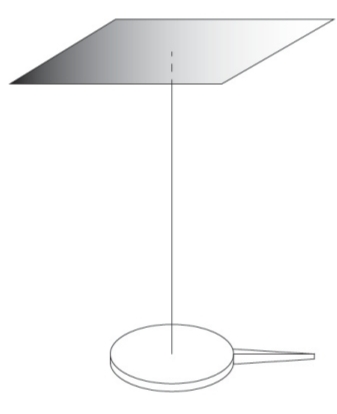
\includegraphics[width=0.35\textwidth, trim={0 3cm 0 0}]{fotocoulomb/pendolotorsione.jpg}
    \end{center}
\end{wrapfigure}

Si fa torcere un filo di $\theta$ attorno al proprio asse, si compie un lavoro che viene 'immagazzinato' nel cilindro come energia potenziale. Possiamo calcolare l'energia potenziale immagazzinata, calcolando il lavoro necessario per farlo ruotare di un angolo $\theta$
\begin{equation}
    W = \int_{0}^{\theta} M d\theta' = \frac{1}{2}k\theta^2    
\end{equation}

Questo cilindro inizierà a oscillare usando quella energia immagazzinata per oscillare. Questa oscillazione si può descrivere attraverso l'equazione differenziale
\begin{equation}
    M = I \frac{d^2 \theta}{dt^2} = -k\theta
\end{equation}
Prendendo la soluzione a questa equazione differenziale e trovando il periodo di oscillazione si ottiene 
\begin{equation}
    T = 2\pi \sqrt{\frac{I}{K}} = 2\pi \sqrt{\frac{LI}{\mu R^4}} \; \; \text{o} \; \; T^2 = 4\pi^2\frac{LI}{\mu R^4}
\end{equation}
Tuttavia, non conosciamo il momento d'inerzia completo del sistema, ma conosciamo quella della corona circolare che può essere montata per oscillare sullo stesso asse del piattello. In questo modo si misura il periodo di oscillazione del piattello scarico e del piattello caricato con le corone circolari che varranno 
\begin{equation}
    T^2_{0,i} = 4\pi^2 \frac{LI_0}{\mu R^4} \; \; \text{e} \; \; T^2_{i} = 4\pi^2 \frac{L(I_0 + I_i)}{\mu R^4}
\end{equation}
e sottraendo queste equazioni si trova l'equazione 
\begin{equation}
    T^2_i - T^2_{0,i} = 4\pi^2 \frac{LI_i}{\mu R^4}
\end{equation}
che permette calcolare il modulo di Coulomb, in quanto si può calcolare il momento d'inerzia della corona circolare. 
\begin{equation}
    \mu = 4\pi^2 \frac{L}{R^4} \frac{I_i}{T_i^2 - T_{0,i}^2}
\end{equation}
Gli oggetti di cui si misureranno il momento d'inerzia sono corone circolari. Questo vuol dire che il loro momento d'inerzia si può calcolare con la formula 
\begin{equation}
    I_c = \frac{M}{2} (R^2_f + R^2_i)
\end{equation}
mentre quello del disco è 
\begin{equation}
    I_d = \frac{1}{2}MR^2
\end{equation}
Tutte queste formule ci permettono di scrivere l'equazione completa per il calcolo del modulo di Coulomb
\begin{equation}
    \mu = 2\pi^2 \frac{L}{(D_F/2)^4} \frac{((D_e/2)^2 + (D_i/2)^2)_i M_i}{T^2_i-T^2_0}
\end{equation}

\subsection{Errori}
Come ricavata nella precedente sezione, il modulo di Coulomb si può calcolare attraverso la formula
\begin{equation}
    \mu = 2\pi^2 \frac{L}{(D_F/2)^4} \frac{((D_e/2)^2 + (D_i/2)^2)_i M_i}{T^2_i-T^2_0}
\end{equation}
Questa si può dividere in due parti, una che non cambiano da misura a misura, 
\begin{equation}
    A = \frac{L}{(D_f/2)^4} \; \; \text{con errore} \; \; \frac{\Delta A}{A} = \frac{\Delta L}{L} + 4\frac{\Delta D_f}{D_f}
\end{equation}
e un altra parte che cambiano per diverse corone circolari di masse diverse
\begin{equation}
    B = \frac{((D_e/2)^2+(D_i/2)^2)_i M_i}{T^2_i - T^2_i-T^2_{i,0}} 
\end{equation}
che, nell'ipotesi che gli errore dominante sia di natura di misura, si calcola
\begin{equation}
    \frac{\Delta B}{B} = \frac{\Delta M_i}{M_i} + \frac{\Delta ((D_e/2)^2+(D_i/2)^2)_i M_i}{((D_e/2)^2+(D_i/2)^2)_i M_i} + \frac{\Delta (T^2_i-T^2_{i,0})}{T^2_i-T^2_{i,0}}
\end{equation}

Se invece gli errori sono dominati da tipo statistici, l'errore si trova usando la legge della propagazione della varianza, ovvero trovando la miglior stima di $B$ usando la media pesata, usando le varianze come pesi, e poi trovando la miglior stima della varianza. 
Alla fine, il modulo di Coulomb avrà errore pari a 
\begin{equation}
    \Delta \mu = \mu (\frac{\Delta A}{A} + \frac{\Delta B}{B})
\end{equation}

\section{Metologia}
\subsection{Apparato Sperimentale}
Come già scritto in precedenza, l'apparato principale per la misurazione del Modulo di Coulomb era il pendolo a torsione costituito da:
\begin{itemize}
    \item supporto per fissare l'estremità del filo
    \item filo di acciaio, disposto verticalmente
    \item piattello appeso al filo 
    \item corone circolari di diverse masse e diversi raggi
\end{itemize}
Per misurare, sono stati usati i seguenti strumenti:
\begin{itemize}
    \item metro lineare (errore di sensibilità di \SI{5E-4}{m})
    \item calibro ventesimale digitale (errore di sensibilità di $\SI{1E-4}{m}$)
    \item calibro palmer digitale (errore di sensibilità di $\SI{1E-4}{m}$)
    \item bilancia digitale (errore di sensibilità di $\SI{1E-3}{g}$)
    \item cronometro digitale (errore di sensibilità di $\SI{1E-2}{s}$)
\end{itemize}

\subsection{Procedimento di Misura}
Innanzitutto, il procedimento inizia con il misurare i vari parametri fissi, come il diametro del filo $D_f$, le masse $M_i$, il diametro esterno $D_e$ e interno $D_i$ delle corone circolare, e infine la lunghezza del filo $L_f$. Dopodiché, per ogni corona circolare, si sono misurati un totale di $\tau = 5T$ cinque oscillazioni 15 volte per ogni corona circolare. Ogni volta che si andava a cambiare la corona, si misurava una volta a piattello scarico $\tau_{0,i}$, per assicurarsi che le misure fossero indipendenti. 

\section{Risultati}
Rapportati, sono i seguenti risultati ottenuti dalle misure. Per la misura del filo, si è ottenuto

\begin{table} [!ht]
    \centering
    \begin{tabular}{|c|c|c|c|}
    \hline
    \multicolumn{4}{|c|}{Diametro Filo} \\
    \hline
    Misura (mm)& Errore & Misura (mm)& Errore \\
    \hline
    0.399 & 0.001 & 0.401 & 0.001 \\
    0.400 & 0.001 & 0.399 & 0.001 \\
    0.399 & 0.001 & 0.397 & 0.001 \\
    0.400 & 0.001 & 0.400 & 0.001 \\
    0.401 & 0.001 & 0.398 & 0.001 \\
    \hline
    \end{tabular}
\end{table}
Prendendo la semisomma dei valori massimi e minimi, si ottiene un valore del diametro del filo di $D_f$ = $0.392\pm{0.001}$mm, mentre per la lunghezza del filo, si è misurato un valore di $L_f$ = $1.18\pm{0.005}$m. Per le corone circolari, si sono raccolti questi dati:
\begin{table}[!ht]
    \centering
    \begin{tabular}{|c|c|c|c|}
    \hline
    Numero Corona & $M_i$ (g)& $D_e$ (mm) & $D_i$ (mm)\\
    \hline    
    1 & 199.12 & 40.01 & 20.23 \\
    2 & 290.80 & 49.05 & 20.21 \\
    3 & 291.73 & 67.36 & 23.83 \\
    4 & 203.12 & 59.87 & 19.92 \\ 
    5 & 211.45 & 79.99 & 19.79 \\
    \hline
    \end{tabular}
\end{table}
\FloatBarrier
Per gli errori si ha che $\Delta M_i = \pm{0.01} \SI{}{g}$, $\Delta D_e = \pm{0.01} \SI{}{mm}$, e $\Delta D_i = \pm{0.01} \SI{}{mm}$. Le misure di $\tau_i$ e $\tau_{i,0}$, per ogni corona sono

\begin{table}[!ht]
    \centering
    \begin{tabular}{|c|c|}
    \hline
    \multicolumn{2}{|c|}{Corona 1} \\
    \hline 
    $\tau_{i,0}$ & $\tau_i$ \\
    \hline
    11.93 & 20.41 \\
    11.80 & 20.24 \\
    11.95 & 20.33 \\
    12.07 & 20.41 \\
    11.96 & 20.32 \\
    11.86 & 20.38 \\
    11.87 & 20.29 \\
    11.93 & 20.29 \\
    11.80 & 20.20 \\
    11.90 & 20.47 \\
    11.84 & 20.27 \\
    11.84 & 20.15 \\ 
    11.86 & 20.32 \\
    11.92 & 20.24 \\
    11.87 & 20.30 \\
    \hline
    \end{tabular}
    \quad
    \begin{tabular}{|c|c|}
    \hline
    \multicolumn{2}{|c|}{Corona 2} \\
    \hline 
    $\tau_{i,0}$ & $\tau_i$ \\
    \hline
    11.95 & 26.47 \\
    11.86 & 26.58 \\
    12.00 & 26.53 \\
    12.06 & 26.47 \\
    11.93 & 26.41 \\ 
    11.80 & 26.40 \\
    11.95 & 26.40 \\
    11.90 & 26.53 \\
    11.90 & 26.64 \\
    11.90 & 26.36 \\
    11.92 & 26.80 \\
    12.00 & 26.52 \\
    11.81 & 26.56 \\
    12.01 & 26.46 \\
    11.96 & 26.50 \\
    \hline
    \end{tabular}
    \quad
    \begin{tabular}{|c|c|}
    \hline
    \multicolumn{2}{|c|}{Corona 3} \\
    \hline 
    $\tau_{i,0}$ & $\tau_i$ \\
    \hline
    11.87 & 33.33 \\
    11.86 & 33.69 \\
    11.80 & 33.90 \\
    11.81 & 33.55 \\ 
    12.01 & 33.58 \\
    11.93 & 33.41 \\
    11.97 & 34.04 \\
    11.90 & 33.63 \\
    11.90 & 34.18 \\
    11.92 & 33.87 \\
    11.86 & 33.83 \\
    11.90 & 34.15 \\
    11.89 & 34.09 \\
    11.85 & 33.93 \\
    12.00 & 34.46 \\
    \hline
    \end{tabular}
    \quad
    \begin{tabular}{|c|c|}
    \hline
    \multicolumn{2}{|c|}{Corona 4} \\
    \hline 
    $\tau_{i,0}$ & $\tau_i$ \\
    \hline
    11.64 & 26.39 \\
    11.72 & 26.15 \\
    11.63 & 26.32 \\
    11.70 & 26.35 \\
    11.51 & 26.36 \\
    11.64 & 26.03 \\
    11.60 & 26.42\\
    11.63 & 26.05\\
    11.64 & 26.07\\
    11.66 & 26.40\\
    11.78 & 26.17\\
    11.64 & 26.21\\
    11.81 & 26.09\\
    11.64 & 26.14\\
    11.72 & 26.29\\
    \hline
    \end{tabular}
    \quad
    \begin{tabular}{|c|c|}
    \hline
    \multicolumn{2}{|c|}{Corona 5} \\
    \hline 
    $\tau_{i,0}$ & $\tau_i$ \\
    \hline
    11.86 & 33.21 \\
    11.64 & 33.50 \\
    11.63 & 33.32 \\
    11.73 & 33.53 \\
    11.96 & 33.76 \\
    11.67 & 33.60 \\
    11.70 & 33.29 \\
    11.84 & 33.43 \\
    11.70 & 33.64 \\
    11.65 & 33.58 \\
    11.63 & 33.41 \\
    11.60 & 33.27 \\
    11.64 & 33.38 \\
    11.69 & 33.49 \\
    11.66 & 33.36 \\
    \hline
    \end{tabular}
\end{table}
\FloatBarrier
Usando la prima corona, abbiamo inoltre misurato i periodi usando due lunghezze diverse. I risultati sono

\begin{table} [!ht]
    \centering
    \begin{tabular}{|c|c|}
    \hline
    \multicolumn{2}{|c|}{$L = 0.717$} \\
    \hline
    $\tau_{i,0}$ & $\tau_i$ \\
    \hline
    9.40 & 21.21 \\
    9.23 & 21.09 \\
    9.40 & 21.15 \\
    9.46 & 21.18 \\
    9.39 & 21.16 \\
    9.45 & 21.15 \\
    9.42 & 21.20 \\
    9.48 & 21.29 \\
    9.43 & 21.21 \\
    9.46 & 21.18 \\
    9.45 & 21.27 \\
    9.35 & 21.40 \\
    9.37 & 21.35 \\
    9.40 & 21.20 \\
    9.38 & 21.06 \\
    \hline
    \end{tabular}
    \quad
    \begin{tabular}{|c|c|}
    \hline
    \multicolumn{2}{|c|}{$L = 0.378$} \\
    \hline
    $\tau_{i,0}$ & $\tau_i$ \\
    \hline
    6.92 & 11.92 \\
    6.76 & 11.96 \\
    6.92 & 11.89 \\
    6.96 & 11.87 \\
    6.81 & 11.87 \\
    6.87 & 11.73 \\
    6.84 & 11.87 \\
    6.89 & 11.90 \\
    6.92 & 11.86 \\
    6.86 & 11.87 \\
    6.90 & 11.69 \\
    6.92 & 11.91 \\
    6.87 & 11.84 \\
    6.88 & 11.90 \\
    6.90 & 11.92 \\
    \hline
    \end{tabular}    
\end{table}
\FloatBarrier

\section{Analisi dei Dati}
Prendendo i dati della sezione precedente, si inizia con trovare il periodo medio $\bar{T}_i$ per ogni corona. I risultati sono rapportati nella seguente tabella
\begin{table}
    \centering
    \begin{tabular}{|c|c|c|c|c|}
        \hline
        Numero Corona & $\bar{T}_{i,0}$ & $\sigma_{\bar{T}_{i,0}}$ & $\bar{T}_{i}$ & $\sigma_{\bar{T}_{i}}$ \\
        \hline
        1 & 2.379 & $\pm{0.004}$ & 4.062 & $\pm{0.004}$ \\
        2 & 2.386 & $\pm{0.004}$ & 5.302 & $\pm{0.006}$ \\
        3 & 2.380 & $\pm{0.003}$ & 6.769 & $\pm{0.016}$ \\
        4 & 2.333 & $\pm{0.004}$ & 4.487 & $\pm{0.005}$ \\
        5 & 2.342 & $\pm{0.005}$ & 6.689 & $\pm{0.008}$ \\
        \hline
    \end{tabular}
\end{table}
\FloatBarrier

Usando le formule già trovate nella sezione 1.2 e 1.3, procediamo a c2alcolare $A$ e $\Delta$ A. Come già detto prima, questo valore rimane costante e quindi basta calcolarlo una volta. Usando i dati rapportati nella sezione 3, otteniamo un valore di A pari a 
\begin{equation}
    A = \SI{8.00E14}{1/m^3} \pm{\SI{1.2E13}{}} \SI{}{1/m^3}
\end{equation}
Passando invece al calcolo di B, questo parametro va calcolato ogni volta perchè dipende dalle caratteristiche di ogni corona circolare. Rapportate sono i valori di B e i errori assoluti e varianza. La varianza viene calcolata con $\sigma_{B_{i}}= \frac{\Delta B_i}{\sqrt{3}}$
\begin{table}[!ht]
    \centering
    \begin{tabular}{|c|c|c|c|}
        \hline
        Numero Corona & $B_i$ & $\Delta B_i$ & $\sigma_{B_{i}}$ \\
        \hline
        1 & $\SI{9.23E-6}{}$ & $\pm{\SI{1.4E-7}{}}$ & $\pm{\SI{8.1E-8}{}}$ \\
        2 & $\SI{9.13E-6}{}$ & $\pm{\SI{1.1E-7}{}}$ & $\pm{\SI{6.4E-8}{}}$\\
        3 & $\SI{9.27E-6}{}$ & $\pm{\SI{1.6E-7}{}}$ & $\pm{\SI{9.2E-8}{}}$\\
        4 & $\SI{9.16E-6}{}$ & $\pm{\SI{1.2E-7}{}}$ & $\pm{\SI{6.9E-8}{}}$\\
        5 & $\SI{9.14E-6}{}$ & $\pm{\SI{0.9E-7}{}}$ & $\pm{\SI{5.2E-8}{}}$\\
        \hline
    \end{tabular}
\end{table}
Per la miglior stima di $B$, si usa la media pesata dei vari $B_i$, dove i pesi sono l'inversa della varianza. La varianza su $B$, sarà la somma dell'inversa delle varianze. 
\begin{equation}
    B = \frac{\sum_{i = 1}^{n} \frac{B_i}{\sigma_{B_{i}}^2}}{\sum_{i = 1}^{n}\frac{1}{\sigma_{B_{i}}^2}} \; \; \; \text{con errore} \; \; \; \sigma_{B} = \sqrt{\frac{1}{\sum_{i =1}^{n}\frac{1}{\sigma_{B_{i}}^2}}}
\end{equation}
Dopo, per trasformare la varianza in errore assoluto, si applica $\Delta B = 3\sigma_B$. Così si ricava un valore di $B\pm{\Delta B}$ di 
\begin{equation}
    B = \SI{9.168E-6}{}\pm{\SI{9.0E-8}{}} 
\end{equation}
Usando $A$ e $B$ nella formula per il Modulo di Coulomb, si ottiene un valore di $\mu \pm{\Delta \mu}$ 
\begin{equation}
    \mu = \SI{1.448E11}{} \pm{\SI{2.6E9}{Pa}}
\end{equation}

\section{Conclusione}
Il valore atteso era di $\mu = \SI{1.3E11}{Pa}$. Il valore trovato è leggermente fuori dal valore atteso. Questo può essere causato da vari fattori come gli errori de sensibilità degli strumenti o anche il fattore umano durante le misurare delle oscillazioni. Gli umani possono essere molto inaccurati a volte, questo può comportare eventuali errori nelle misure. Inoltre le vibrazioni del tavolo potrebbe affliggere le misurazioni. Essendo in molti gruppi a fare lo sperimento nello stesso laboratorio, potrebbe essere che diverse persone sono scontrate contro il tavolo causando delle piccole vibrazioni. Questo potrebbe causare oscillazioni indesiderate, cambiando i risultati. 

\newpage
\section{Figure}
\subsection{Grafici}
\begin{figure}[!ht]
    \centering
    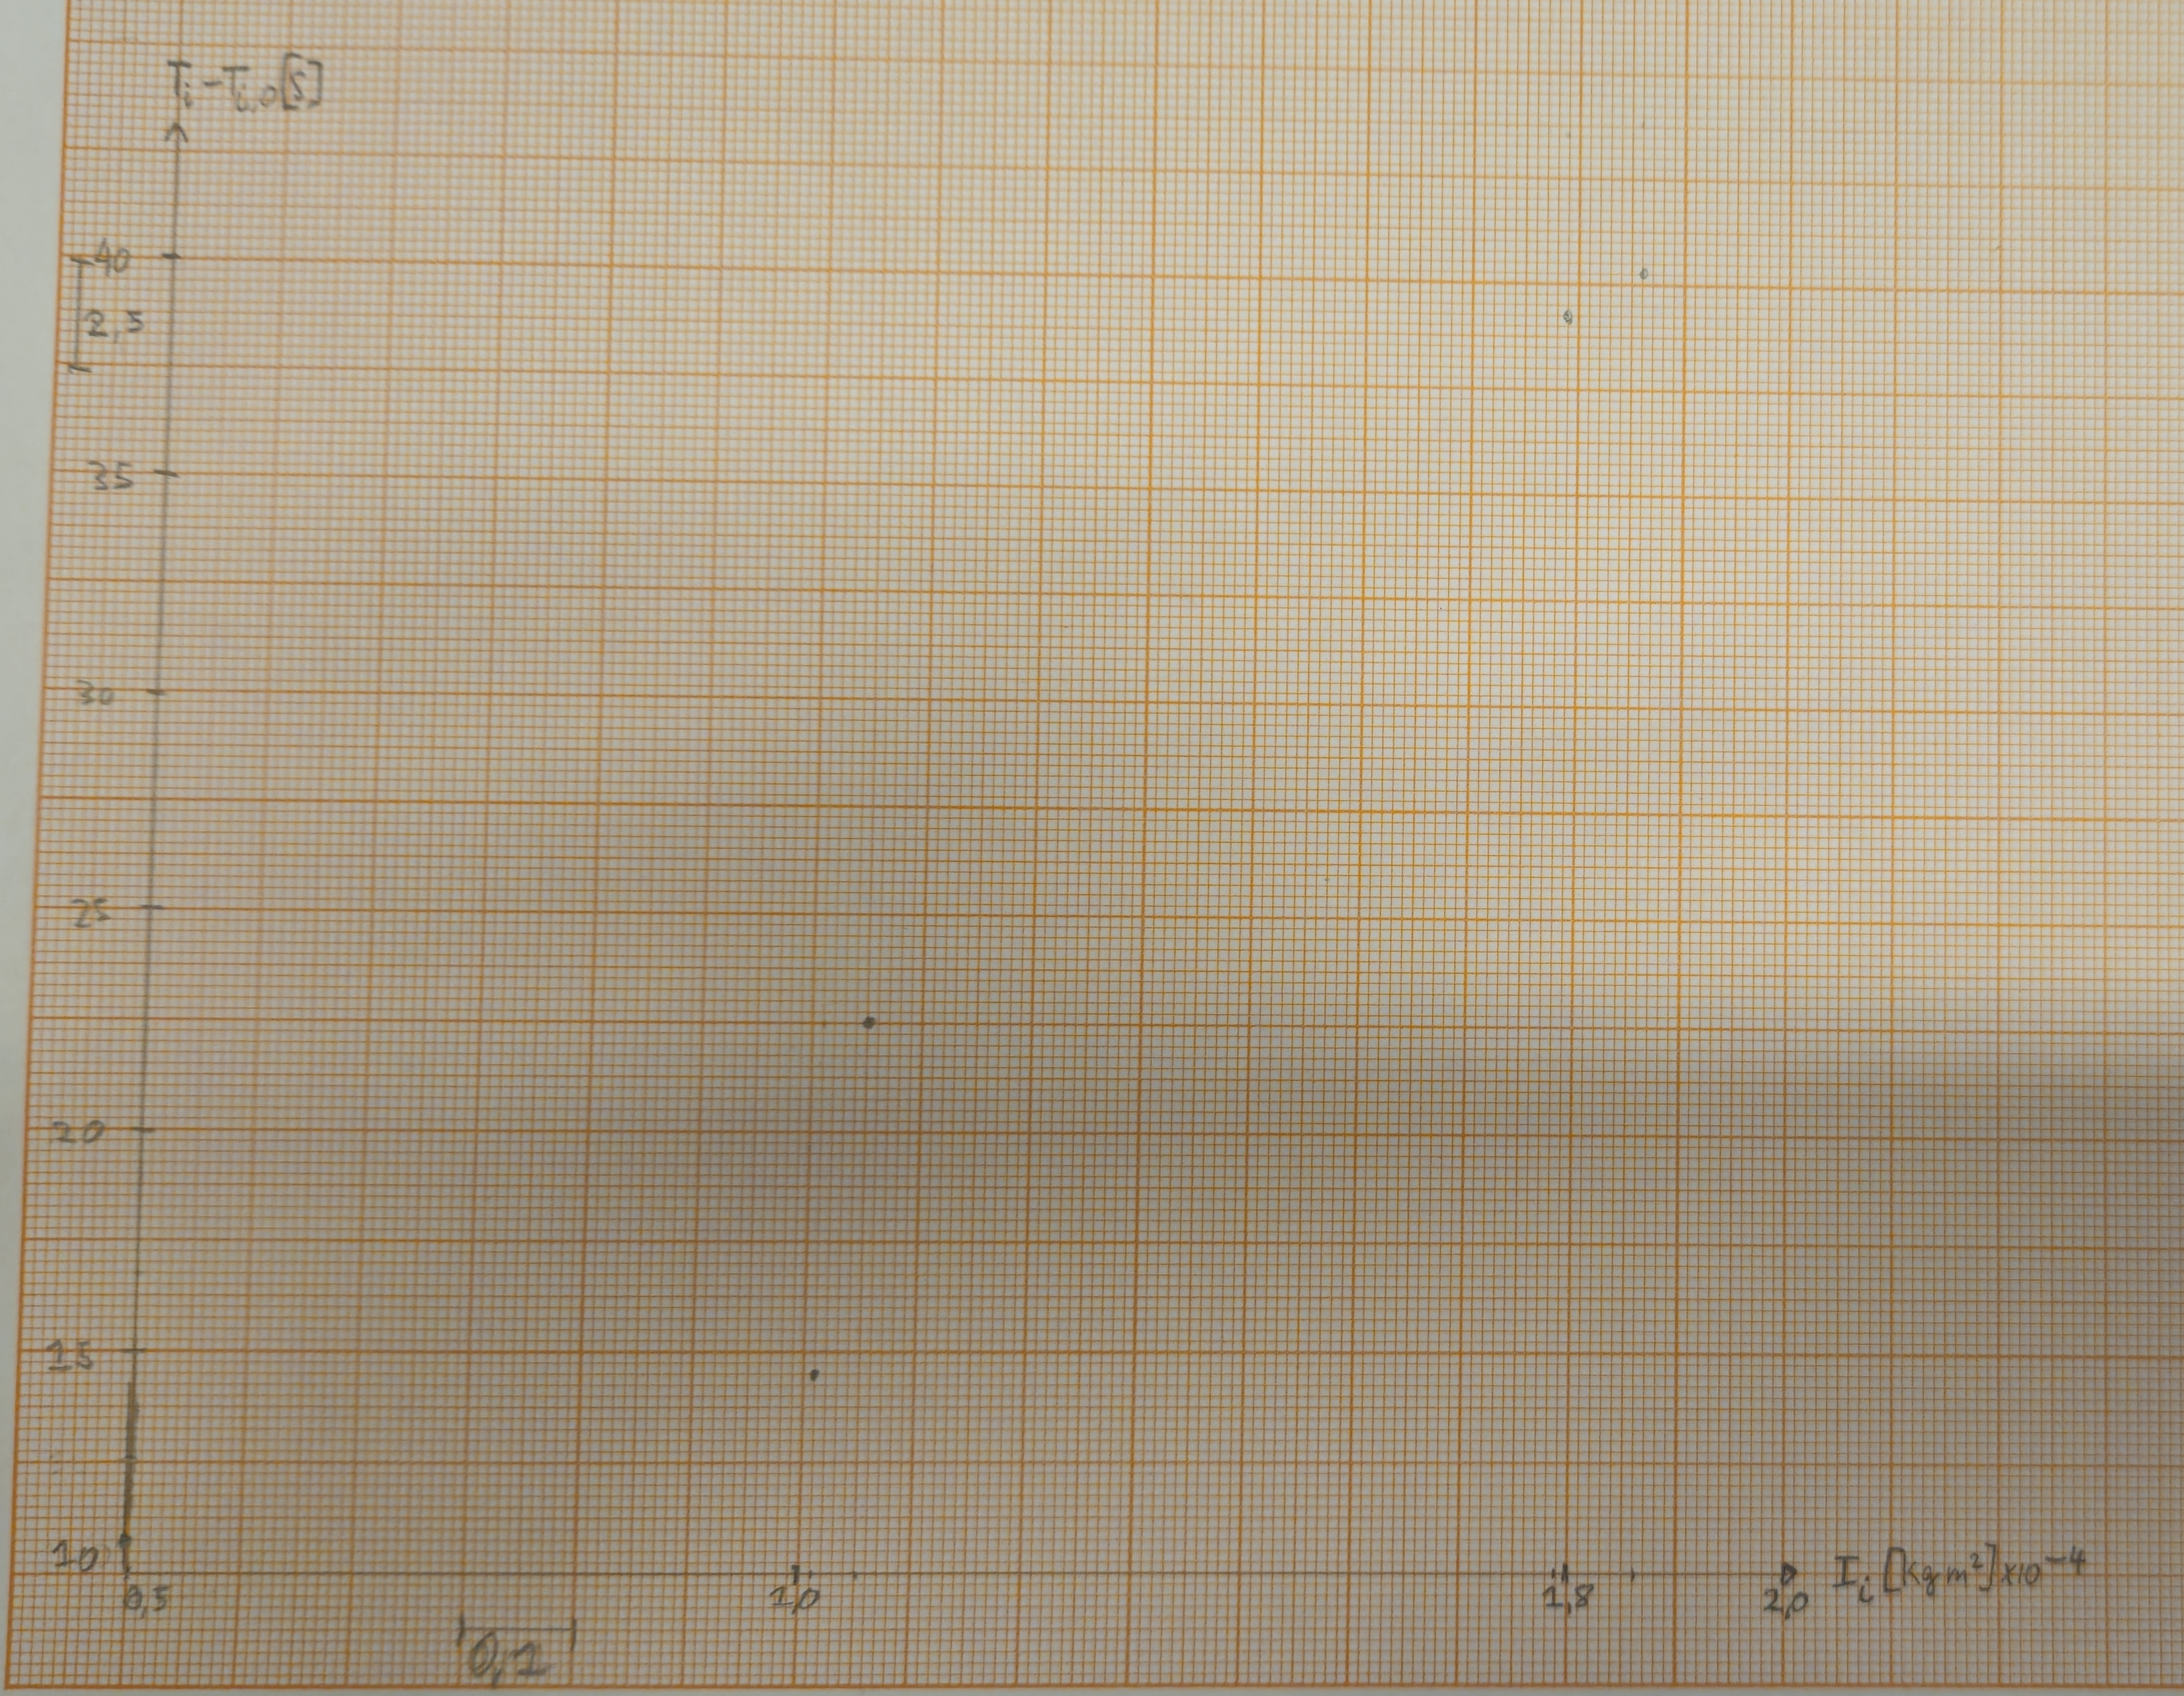
\includegraphics[width=\textwidth]{fotocoulomb/modulocoulomb_TI.jpg}
    \caption{Grafico di $T_i-T_{i,0}$ vs $I_i$}
\end{figure}

\begin{figure}[!ht]
    \centering
    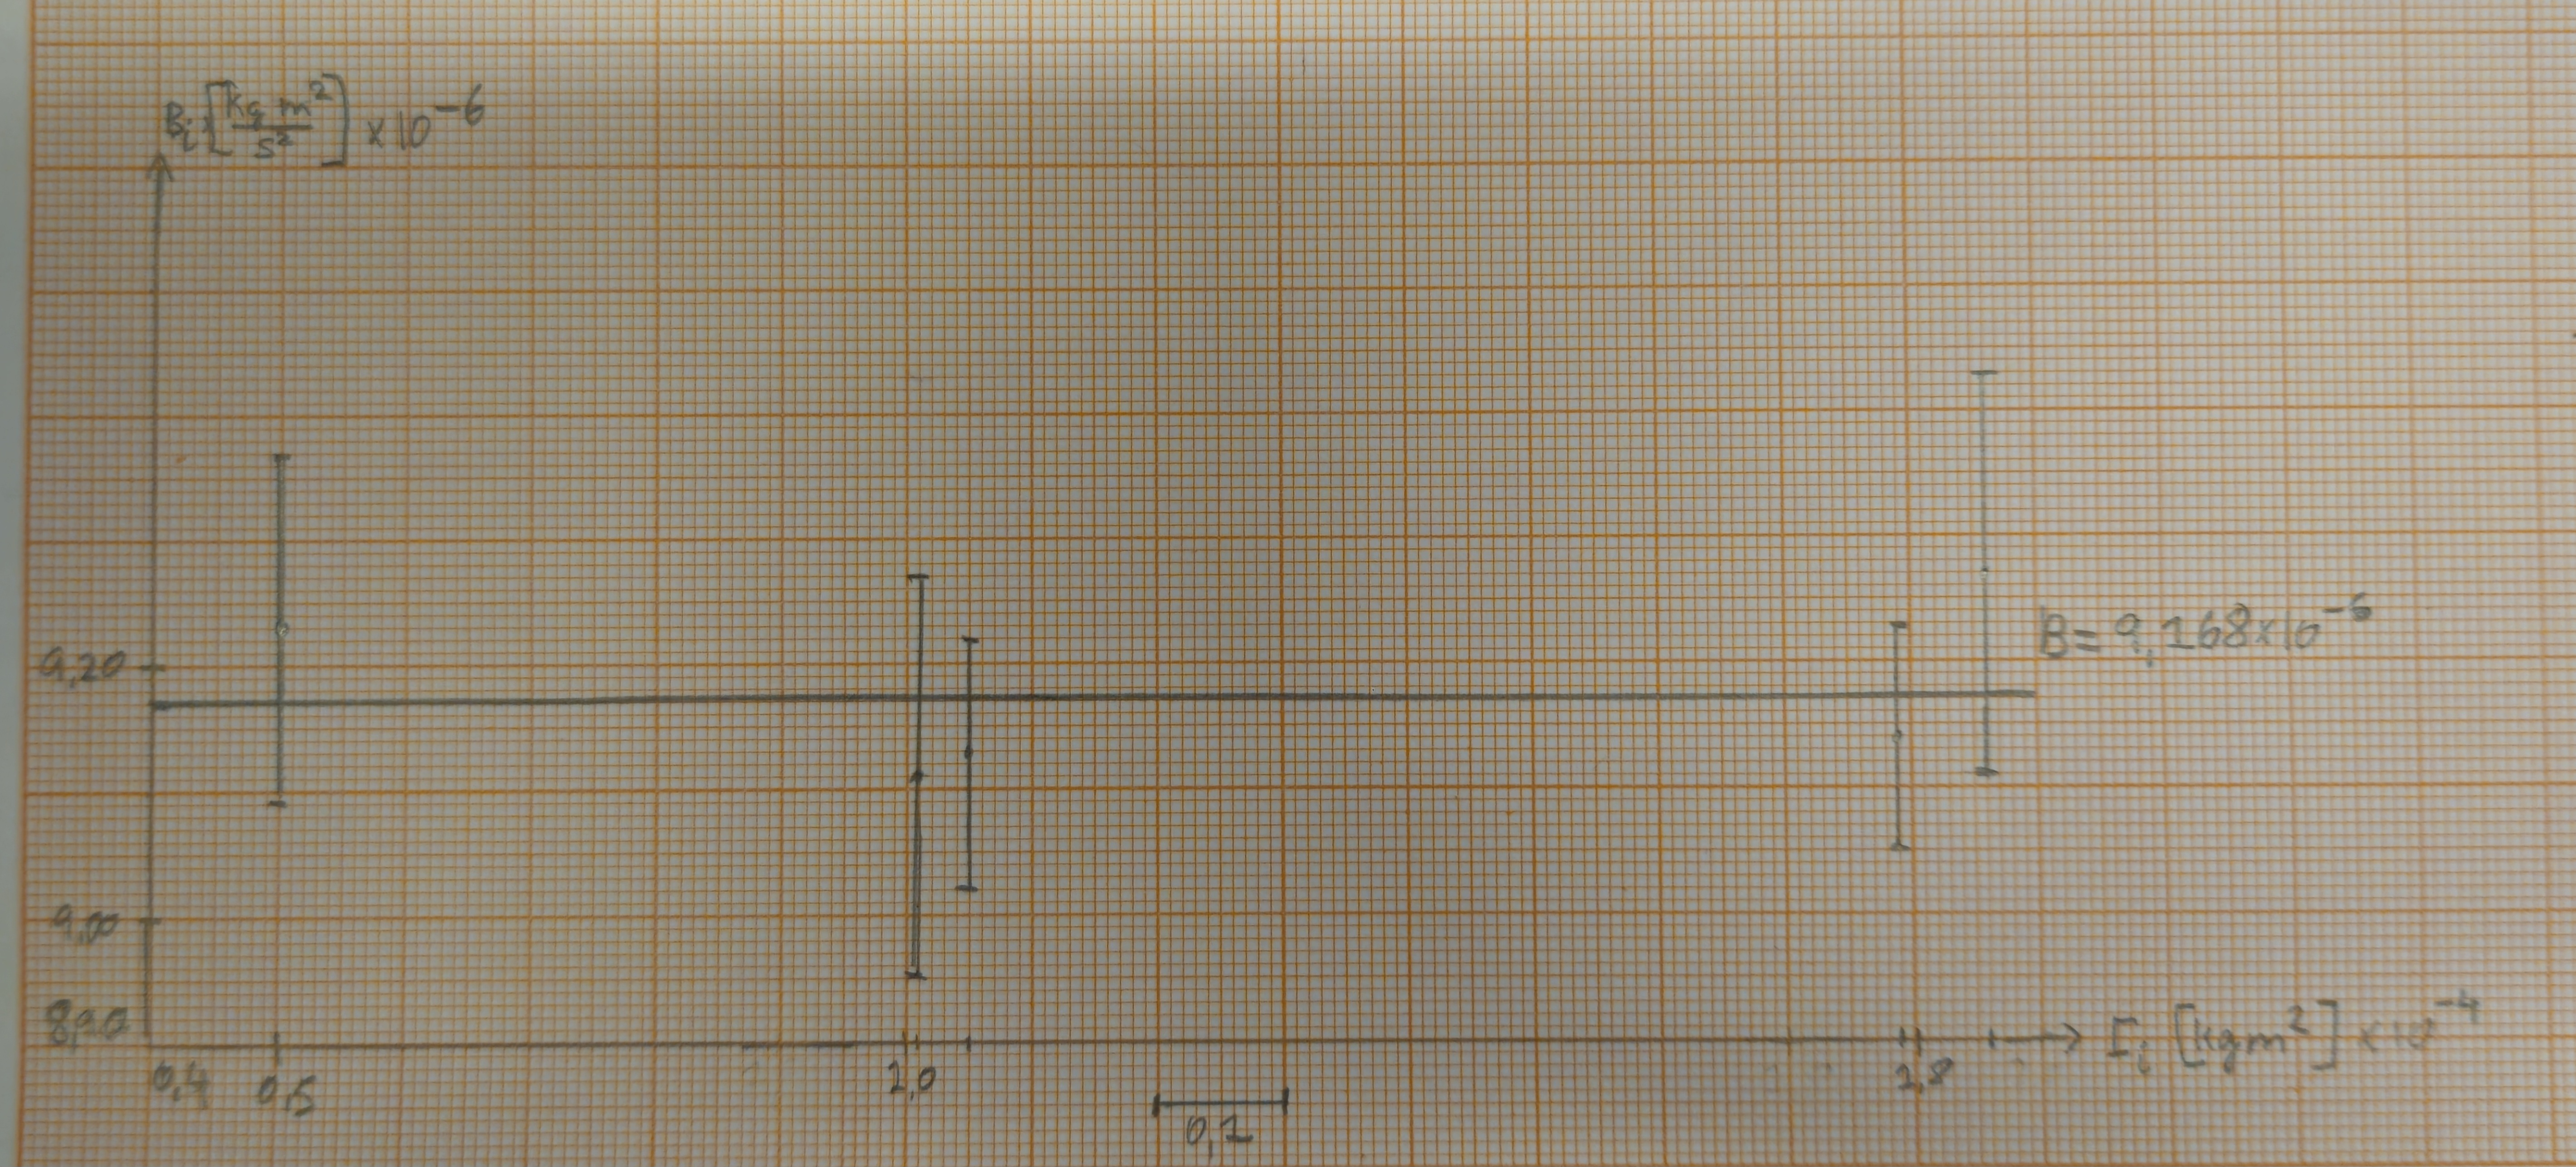
\includegraphics[width=\textwidth]{fotocoulomb/modulocoulomb_BI.jpg}
    \caption{Grafico di $B_i$ vs $I_i$}
\end{figure}


\end{document}
